\documentclass[12pt,a4paper]{article}
\usepackage[legalpaper, portrait, margin=3cm]{geometry}
\usepackage{fancyhdr}
\usepackage{amsmath}
\usepackage{amssymb}
\usepackage{graphicx}
\usepackage{wrapfig}
\usepackage{blindtext}
\usepackage{hyperref}
\usepackage{tikz}
\usepackage{subcaption}

\graphicspath{ {./} }
\hypersetup{
  colorlinks=true,
  linkcolor=blue,
  filecolor=magenta,
  urlcolor=blue,
  citecolor=blue,
  pdftitle={Relatório ASA Projeto 2 2021/2022},
  pdfpagemode=FullScreen,
}

\pagestyle{fancy}
\fancyhf{}
\rhead{Grupo \textbf{al007}}
\lhead{Relatório Projeto 2 ASA 2021/2022 LEIC-A}
\cfoot{Diogo Correia (99211) e Tomás Esteves (99341)}

\definecolor{pastel-green}{HTML}{CBE896}
\definecolor{pastel-yellow}{HTML}{FEE440}

\renewcommand{\footrulewidth}{0.2pt}

\renewcommand{\labelitemii}{$\circ$}
\renewcommand{\labelitemiii}{$\diamond$}

\begin{document}
  \section{Descrição do Problema e da Solução}

  Pretende-se encontrar, dada uma árvore geneológica e dois nós, os \textbf{ancestrais comuns mais próximos} de ambos os nós.

  Para resolver o \textbf{problema} utilizou-se uma lista de nós.
  Um nó é composto pela identificação dos seus pais e pelo número de filhos que tem.
  Para otimizar a utilização de memória, apenas é guardado o número de filhos, não quais são, visto que estes não são necessários à resolução do problema.
  Ao decorrer da solução, trabalhamos maioritariamente no grafo transposto, que tem a vantagem de cada nó ter, no máximo, dois arcos.

  O primeiro passo é verificar que o input dado é uma árvore geneológica válida.
  Para tal, é feito o seguinte:
  
  \begin{itemize}
    \setlength{\itemsep}{0pt}
      \item Ao ler o input verifica-se se um nó tem mais de 2 pais. Caso tenha, a árvore é inválida.
      \item Depois de ser lido o input todo, realiza-se uma DFS e no caso de se detetar que existe uma aresta que toca num nó já aberto mais ainda não fechado (\texttt{GREY}), sabe-se que existe um loop, pelo que a árvore é inválida.
  \end{itemize}

  Caso a árvore seja inválida, o programa escreve "\texttt{0}" e termina.

  Considerando como exemplo a árvore na \textit{Fig. 1(a)}, realizam-se duas \textbf{BFS}, começando em cada um dos dois nós do input (no exemplo, os nós \texttt{5} e \texttt{6}).
  Ao visitar cada nó da árvore, incrementa-se o contador de cada nó.
  No fim da execução das duas BFS, temos que os nós com o contador com valor igual a \texttt{2} são os ancestrais comuns a ambos os nós de início.
  Na \textit{Fig. 1(b)} vemos o resultado final da execução da BFS em ambos os nós, em que os nós a verde são os que têm contador a 2, os nós a amarelo têm o contador a 1, e os nós a cizento têm o contador a 0.

  \begin{figure}[h]
    \centering
    \begin{subfigure}[t]{0.4\linewidth}
      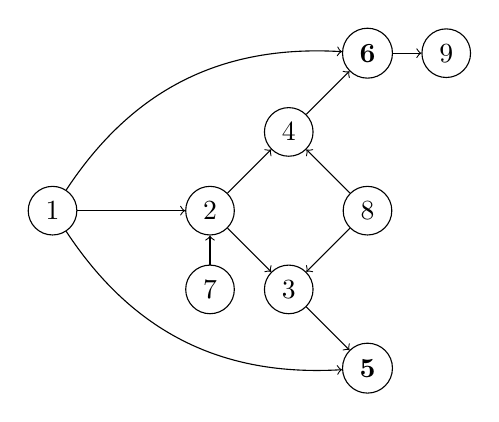
\begin{tikzpicture}[nodes={draw, circle}, ->]
        \node (a1) at (-7,5) {1};
        \node (a2) at (-5,5) {2};
        \node (a3) at (-4,4) {3};
        \node (a4) at (-4,6) {4};
        \node (a5) at (-3,3) {\textbf{5}};
        \node (a6) at (-3,7) {\textbf{6}};
        \node (a7) at (-5,4) {7};
        \node (a8) at (-3,5) {8};
        \node (a9) at (-2,7) {9};

        \draw (a1) -> (a2);
        \draw (a2) -> (a3);
        \draw (a2) -> (a4);
        \draw (a3) -> (a5);
        \draw (a4) -> (a6);
        \path (a1) edge [bend right] (a5);
        \draw (a1) edge [bend left] (a6);
        \draw (a7) -> (a2);
        \draw (a8) -> (a3);
        \draw (a8) -> (a4);
        \draw (a6) -> (a9);
      \end{tikzpicture}
      \caption{Antes da execução nos nós 5 e 6} \label{fig:M1}
    \end{subfigure}
    \qquad
    \begin{subfigure}[t]{0.4\linewidth}
      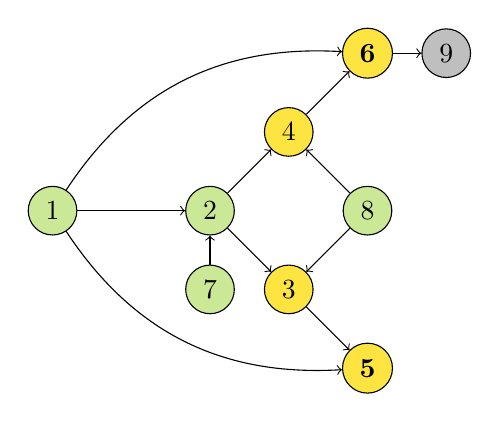
\begin{tikzpicture}[nodes={draw, circle}, ->]
        \node[fill=pastel-green] (a1) at (-7,5) {1};
        \node[fill=pastel-green] (a2) at (-5,5) {2};
        \node[fill=pastel-yellow] (a3) at (-4,4) {3};
        \node[fill=pastel-yellow] (a4) at (-4,6) {4};
        \node[fill=pastel-yellow] (a5) at (-3,3) {\textbf{5}};
        \node[fill=pastel-yellow] (a6) at (-3,7) {\textbf{6}};
        \node[fill=pastel-green] (a7) at (-5,4) {7};
        \node[fill=pastel-green] (a8) at (-3,5) {8};
        \node[fill=lightgray] (a9) at (-2,7) {9};

        \draw (a1) -> (a2);
        \draw (a2) -> (a3);
        \draw (a2) -> (a4);
        \draw (a3) -> (a5);
        \draw (a4) -> (a6);
        \path (a1) edge [bend right] (a5);
        \draw (a1) edge [bend left] (a6);
        \draw (a7) -> (a2);
        \draw (a8) -> (a3);
        \draw (a8) -> (a4);
        \draw (a6) -> (a9);
      \end{tikzpicture}
      \caption{Após execução de BFS. Nós a verde são os ancestrais comuns.} \label{fig:M2}
    \end{subfigure}
    \caption{Descoberta de todos os ancestrais comuns.}
  \end{figure}

  \begin{wrapfigure}{r}{0.4\textwidth}
    \centering
    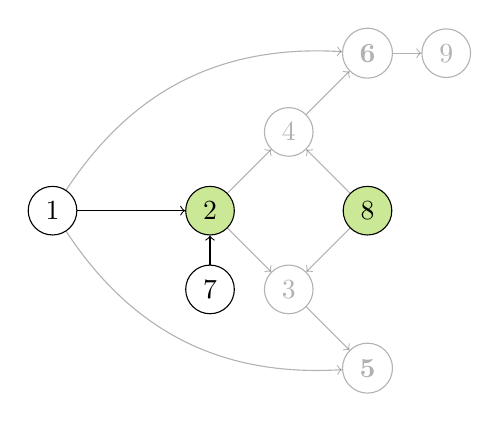
\begin{tikzpicture}[nodes={draw, circle}, ->]
      \node (a1) at (-7,5) {1};
      \node[fill=pastel-green] (a2) at (-5,5) {2};
      \node[opacity=0.3] (a3) at (-4,4) {3};
      \node[opacity=0.3] (a4) at (-4,6) {4};
      \node[opacity=0.3] (a5) at (-3,3) {\textbf{5}};
      \node[opacity=0.3] (a6) at (-3,7) {\textbf{6}};
      \node (a7) at (-5,4) {7};
      \node[fill=pastel-green] (a8) at (-3,5) {8};
      \node[opacity=0.3] (a9) at (-2,7) {9};
  
      \draw (a1) -> (a2);
      \draw[opacity=0.3] (a2) -> (a3);
      \draw[opacity=0.3] (a2) -> (a4);
      \draw[opacity=0.3] (a3) -> (a5);
      \draw[opacity=0.3] (a4) -> (a6);
      \path[opacity=0.3] (a1) edge [bend right] (a5);
      \draw[opacity=0.3] (a1) edge [bend left] (a6);
      \draw (a7) -> (a2);
      \draw[opacity=0.3] (a8) -> (a3);
      \draw[opacity=0.3] (a8) -> (a4);
      \draw[opacity=0.3] (a6) -> (a9);
    \end{tikzpicture}
    \caption{Árvore resultante e resultado final}
  \end{wrapfigure}

  De seguida, eliminam-se os nós que não são ancestrais comuns, ou seja, todos os nós com contador inferior a \texttt{2}.
  Podemos concluir que todos os nós que não têm filhos na árvore resultante são os ancestrais comuns mais próximos. No exemplo acima, correspondem aos nós \texttt{2} e \texttt{8}, tal como ilustrado na \textit{Fig. 2}.

  Por fim, são percorridos todos os nós por ordem crescente, e o programa escreve o índice de todos os nós ancestrais comuns mais próximos, isto é, os nós que têm o contador a \texttt{2} e não tenham filhos na árvore resultante.
  Caso não exista nenhum nó nesta situação, o programa escreve "\texttt{-}" e termina.

  \section{Análise Teórica}

  Seja $V$ o número de nós e $E$ o número de arestas.

  \begin{itemize}
    \setlength{\itemsep}{0pt}
    \item Começa-se por ler o input.
    \begin{itemize}
      \setlength{\itemsep}{0pt}
      \item A inicialização da lista de nós é feita em tempo linear, $\Theta(V)$.
      \item De seguida, efetua-se a leitura das arestas, que são adicionadas aos vértices a que pertencem.
      Caso se detete um nó com mais de dois pais, o programa termina imediatamente. Logo, $O(E)$.
    \end{itemize}

  \item É efetuada uma DFS para detetar ciclos na árvore dada como input. Logo, $O(V + E)$.

  \item São efetuadas duas BFS para detetar os ancestrais comuns dos dois nós, incrementando o contador dos nós encontrados. Logo, $O(V + E)$.

  \item Remover todas as arestas que ligam nós na árvore resultante dos ancestrais comuns. Logo, $\Theta(V)$.

  \item Imprimir todos os nós que são ancestrais comuns mais próximos. Logo $\Theta(V)$.
  \end{itemize}

  Logo, no pior caso tem-se uma complexidade temporal $O(V + E)$.

  A solução tem complexidade espacial $\Theta(V)$, visto que se utilizou apenas uma lista de tamanho dos números de nós.

  \section{Avaliação Experimental dos Resultados}

  Foram criadas instâncias de input com probablidade de criar aresta de 99\% (pior caso), para valores de nós ($V$) entre 10 e 1 000 000. Para cada ordem de grandeza foram gerados no máximo 100 inputs, para um total de 451 inputs.
  O programa foi executado, pelo menos 100 vezes para cada input, recorrendo ao programa \href{https://github.com/sharkdp/hyperfine}{\textit{hyperfine}}.
    
  \begin{figure}[h]
    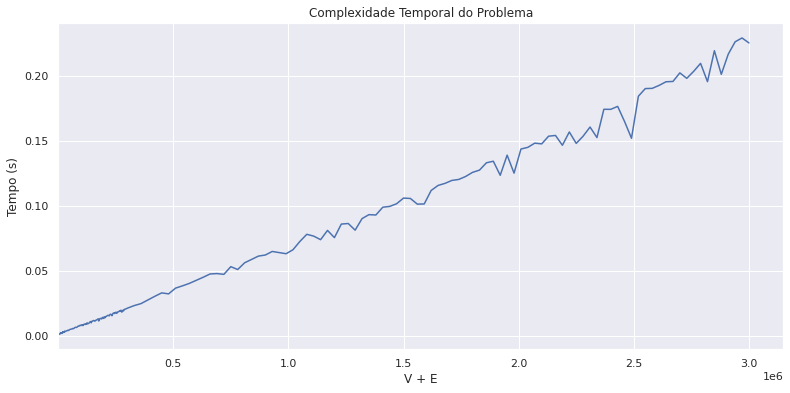
\includegraphics[width=1\textwidth]{report.png}
    \caption{Tempo de execução do programa em segundos, em função do tamanho do input}
  \end{figure}
  
  O gráfico apresentado tem uma escala $V + E$ no eixo dos $xx$ e o tempo em segundos no eixo dos $yy$.\\
  Os dados revelam uma reta (relativamente) linear, comprovando que a complexidade temporal do problema é, num caso geral, $O(V + E)$, tal como concluído na análise teórica.

\end{document}
